\documentclass[notitlepage]{article}

\usepackage{amsmath}
\usepackage{titling}
\usepackage{graphicx}
\usepackage[margin=1.5in]{geometry}
\usepackage{cite}
\usepackage{subcaption}


\graphicspath{{figures/paper/final/}{figures/paper/preliminary/}}

\title{Cognitive Mechanisms for Reinforcement Learning Refinement}

\author{
  Krueger, Paul\\
  \texttt{pmk@berkeley.edu,\ \#26969749}
  \and
  Daniels, Dylan\\
  \texttt{dylandaniels@berkeley.edu,\ \#29655144}
}
\date{\today}

\begin{document}

\maketitle

\begin{abstract}
blah blah blah we need to put stuff here.
\end{abstract}

\section*{Introduction}

Reinforcement learning (RL) studies how agents behave to maximize rewards, and has been applied to model human and animal decision making for decades. In addition to providing an algorithmic framework for understanding decision making, there is also strong evidence that RL is implemented in the brain~\cite{daw2005uncertaintyl}. This field of study has identified two general classes of RL employed during decision making and implemented in the brain: model-free RL which assigns values to actions based on simple trial-and-error learning, and model-based RL which represents values of states based on an internal model of the environment. While model-free RL is computationally cheap and efficient, it fails to exploit causal regularities that may be present in the reward structure of the environment. Model-based RL, on the other hand, may lead to more optimal behavior in structured environments, but is computationally expensive.

Usually, these two RL systems are treated as two independent systems, interacting only insofar as they compete for control of behavior~\cite{dolan2013goals}. Indeed, recent evidence suggests that humans employ both types of RL strategies: computationally-efficient but suboptimal heuristic and more optimal but computationally expensive ones~\cite{wilson2014human}, and that they tradeoff between the two~\cite{wilson2015tradeoff}. However,~\cite{sutton1998reinforcement} propose a "DYNA" architecture in which the two systems cooperate: a model-based system is used to simulate past experience in order to update the model-free representations of state-action values. While very little work has been done testing this framework on humans, recent data from human decision making is consistent with DYNA~\cite{gershman2014retrospective}. An open question for research is how these two systems may interact cooperatively~\cite{gershman2015reinforcement}, mediating the tradeoff between optimal representations of the environment and computational efficiency.

DYNA is one means of managing cooperation between these systems, using past experience to reshape values represented by the model-free RL system. Another framework for using a model-based system to guide a model-free system is known as gamification~\cite{mcgonigal2011reality}. Gamification adds pseudorewards to decisions in a non-game context, and can be used to align myopic reward-seeking behavior with longer-term reward maximization. Essentially, it is a way to shape the reward structure of the model-free RL system so that it converges to optimal behavior more quickly, by making myopic decisions globally optimal. While a framework exists for computing optimal pseudorewards~\cite{ng1999policy}, humans might feasibly compute heuristic pseudorewards, and recent evidence shows that humans can effectively apply pseudorewards to improve decision making~\cite{lieder2016helping}.

In this study we examine all three types of RL: a version of model-free RL called Q-learning, DYNA learning, which combines model-free Q-learning and model-based RL, and pseudorewards, which also use a model-based system to modify the reward structure used by Q-learning. Our environment consists of a maze with an agent taking steps to navigate toward a rewarding goal state. Spatial navigation in maze environments has been been studied extensively in psychology and neuroscience for decades, and research has shown that the same neural structures underlying spatial maps also provide a basis for episodic memory and may more generally represent cognitive maps~\cite{o1978hippocampus}. Our results provide a benchmark by which to compare these three learning processes, and future work may be done to test which strategies are employed by human decision makers algorithmically, and how they may be implemented biologically in the brain.

\section*{Methods}

\begin{figure}
\centering
\begin{subfigure}{.4\textwidth}
  \centering
  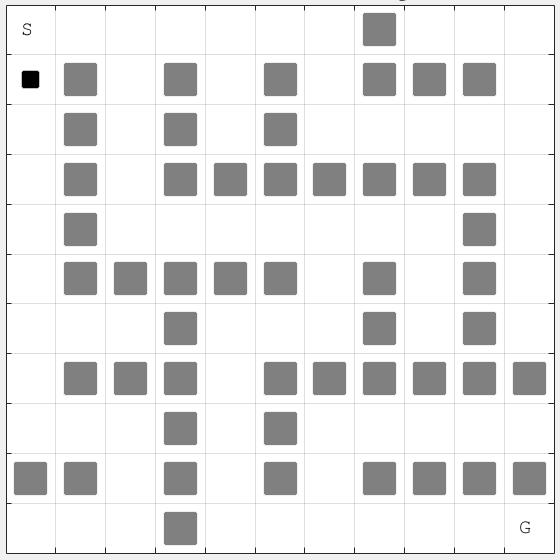
\includegraphics[width=.95\linewidth]{dense_maze}
  \caption{The dense maze.}
\end{subfigure}
\begin{subfigure}{.4\textwidth}
  \centering
  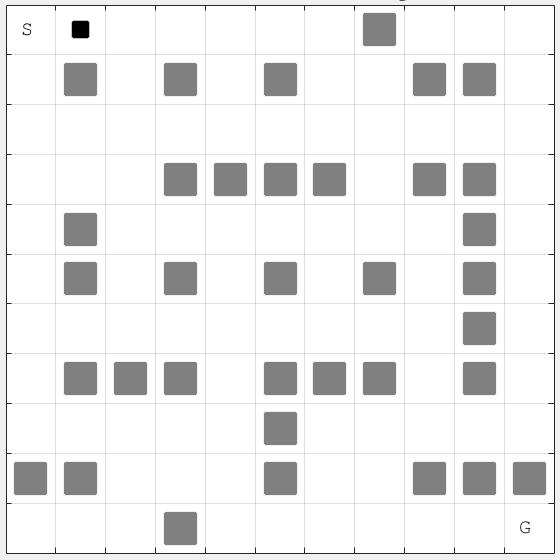
\includegraphics[width=.95\linewidth]{sparse_maze}
  \caption{The sparse maze.}
\end{subfigure}
\caption{Two variants of the maze game. The square labelled ``S'' is the agent's start state, and the square labelled ``G'' is the goal state. The black box is the agent. The gray squares are wall obstacles.}
\label{fig:mazes}
\end{figure}

To explore theories about reinforcement learning in cognition, we constructed a simple two-dimensional maze game whereby an agent was tasked with learning how to reach a terminal goal state from a start state. The terminal goal state confers the agent a reward of 1 point, and resets the agent's location to the starting point (Figure 1). We study two different mazes: a \textit{dense} maze (Figure 1a) and a \textit{sparse} maze (Figure 1b). The sparse maze is easier for the agent to solve, but it is also easier for the agent to get stuck in a suboptimal path. The dense maze, on the other hand, has only one clear path to the solution; as a result, we expect heuristic-based pseudorewards to often fail to find the optimal path.

All of our methods are based on a common model-free reinforcement learning paradigm known as Q-learning~\cite{sutton1998reinforcement}, which learns an optimal policy $\pi^*$ over time. Let $\mathcal{S}$ be the set of states and let $\mathcal{A}$ be the set of actions. For each $(s,a) \in \mathcal{S} \times \mathcal{A}$, a value $Q(s,a)$ is learned via the following algorithm. Initially all $Q(s,a)$ are zero. At each state $s$, with probability $1 - \epsilon$, the agent chooses the action $a \in \mathcal{A}$ with the highest value $Q(s,a)$. With probability $\epsilon$ it chooses an action uniformly at random ($\epsilon$ is a hyperparameter that calibrates the explore-exploit tradeoff). Then, after completing the selected action $a$, the agent moves to $s'$ and updates $Q$ by

\begin{equation}
Q(s,a) \leftarrow Q(s,a) + \alpha (R(s, s') + \gamma \max_{a'} Q(s', a') - Q(s,a))
\label{eq:q-learn}
\end{equation}

where $\alpha$ is the learning rate, $R(s, s')$ is the reward received at state $s'$, and $\gamma$ is the discount factor on rewards. Q-learning will converge with probability one to the optimal policy. 

For our maze game, each state $s$ is a square in the matrix, and each available action $a$ is selected from up the four cardinal directions which do not move the agent into a wall. 

\subsection*{DYNA Planning}

Using the DYNA framework described in~\cite{sutton1998reinforcement}, we can improve upon the naive Q-learning algorithm by recalling a random set of past moves after each step. From a cognitive science perspective, this type of optimization is interesting because it is as if we are replaying past memories. In other words, is it cognitively advantageous to think about past experiences, and as a result, learn more from them? 

Planning is implemented by re-updating $p$ Q-values randomly at the end of each step using Equation~\ref{eq:q-learn}. Only the most recent action for each state is updated, so DYNA planning favors recency.

\subsection*{Pseudorewards}

Pseudorewards are an intelligible way of conferring extra information to an agent about the reward landscape. Essentially, a small reward is given to the Q-learner whenever they take an action that helps the agent move towards the goal. Pseudorewards are defined by \textit{shaping functions} $F$. Instead of the agent receiving actual reward $R(s, s')$ when moving from state $s \rightarrow s'$, the agent receives an augmented reward $R'(s, s')$ where
\begin{equation}
R'(s, s') = R(s, s') + F(s, s')
\end{equation} 

 In~\cite{ng1999policy}, conditions for which the optimal policy $\pi^*$ remains invariant under a \textit{shaping function} are developed. If the shaping function does not possess this invariance policy, it is possible that Q-learning will converge to a suboptimal solution. The simplest example of an invariant shaping function uses the difference in optimal values between the agent's current state and next state:
\begin{equation}
F(s, s') = \gamma V_{\pi^*}(s') - V_{\pi^*}(s) 
\end{equation}
\begin{equation}
V_{\pi^*}(s) =  \max_{a} R(s, s') + \gamma V_{\pi^*}(s')
\end{equation}
We call this method the \textit{optimal policy pseudoreward}--it encourages the agent to always move down the optimal path from its current state. If $\epsilon = 0$, the agent would move directly to the goal along the shortest path.

While the \textit{optimal policy pseudoreward} performs well in practice, it's a bit unrealistic for the agent to have such a complete information set in most applications. To compute the optimal policy, the agent must solve a linear program and have full information about states, actions, transitions, and goal states. A more realistic set of pseudorewards can be derived by approximating the distance to the goal. Intuitively, this corresponds to the agent generally knowing which direction to move in. We call this the \textit{Manhattan pseudoreward}.

\begin{figure}[ht]
\centering
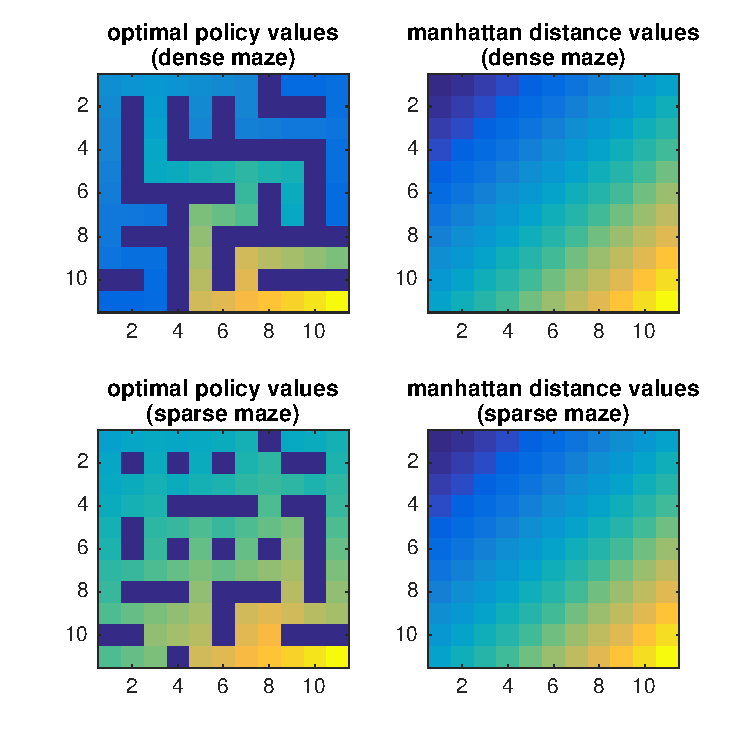
\includegraphics[width=0.8\textwidth]{value_landscapes}
\caption{The landscape of pseudorewards for each maze and each pseudoreward type. Pseudorewards are concocted so that the agent is incentivized to move towards the goal state in the lower rightmost square.}
\label{fig:value-landscapes}
\end{figure}

For our maze environment, we use a modified Manhattan distance metric to implement distance-based pseudorewards. We define the Manhattan distance metric as $\Phi(s) = \gamma^T$, where $T$ is the Manhattan distance, to form the pseudoreward
\begin{equation}
F(s, s') = \gamma \Phi(s') - \Phi(s)
\end{equation} 
which fulfills the conditions in~\cite{ng1999policy} to be an invariant reward transformation. A comparison of the pseudoreward landscape for each of the types of the pseudorewards considered is shown in Figure~\ref{fig:value-landscapes}.

In addition, we also test the sensitivity of both pseudoreward methods to additive white noise. For each pseudoreward $F(s, s')$ conferred, let
\begin{equation}
\tilde{F}(s, s') = F(s, s') + e_t
\end{equation} 

\noindent where $e_t \sim N(0, \sigma^2)$. The larger the value of $\sigma$, the more noisy the pseudoreward $\tilde{F}$. In general pseudorewards $\tilde{F}$ will not lead to invariant policies.

\section*{Experiments}

To analyze the performance of our agent in each of our two maze environments (\textit{dense} and \textit{sparse}), we ran 100 simulations of reinforcement learning for each condition. In each simulation, we allowed the agent to learn for 50 episodes, where each episode entails a series of actions beginning at the start state and terminating at the goal state; the agent automatically advanced to the next episode without reward if a maximum of 2000 steps was reached. For all of our experiments, we set the learning rate $\alpha = 0.1$, the exploratory probability $\epsilon = 0.25$, and the discount factor $\gamma = 0.95$. 

\begin{figure}[ht]
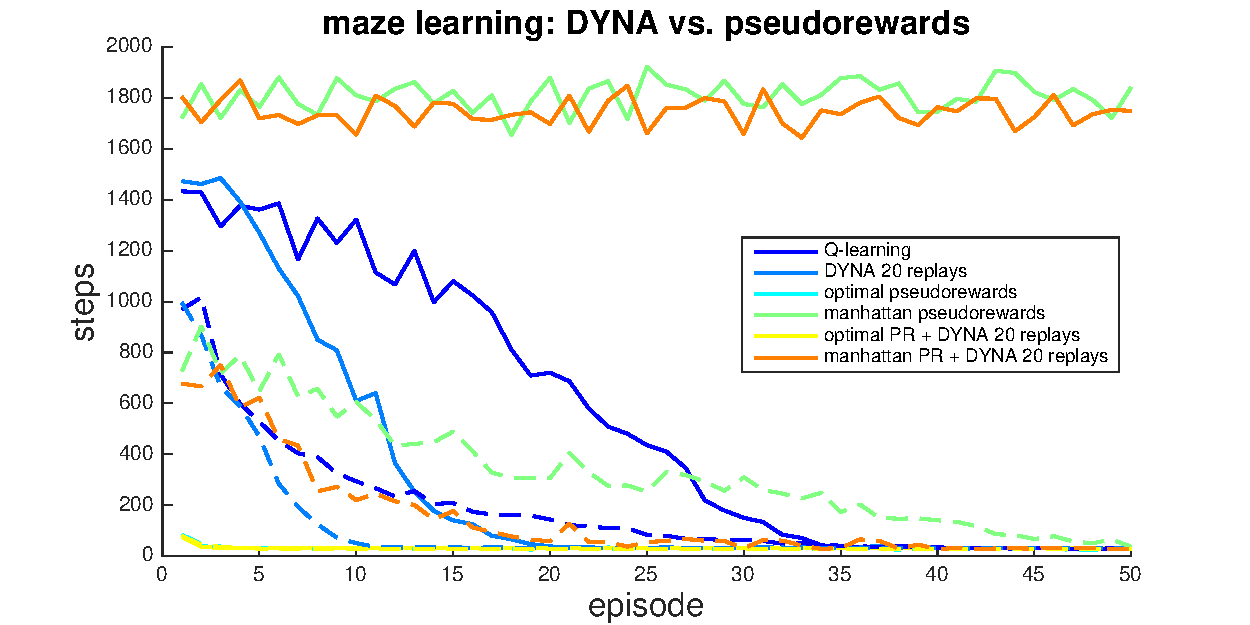
\includegraphics[width=\textwidth]{modelCompareNoNoise}
\caption{The mean number of steps taken for each episode are plotted above for Q-learning and 5 variants, for both the dense maze (shown in solid lines) and the sparse maze (shown in dashed lines). The means are taken over 100 simulations of 50 episodes.}
\label{fig:model-compare}
\end{figure}

As a first pass, we compare the DYNA architecture with $p =20$ replays with the optimal policy and Manhattan pseudoreward architectures (Figure~\ref{fig:model-compare}). For the sparse maze, shown in dashed lines, all methods converge to the optimal number of steps: 20. For the dense maze, the optimal number of steps is 24 and all methods converge except the Manhattan distance-based pseudoreward. This is because in the dense maze (shown in Figure~\ref{fig:mazes}), it is very easy for the agent to get stuck following a false pseudoreward path towards the goal: the agent keeps butting up against a wall on the lower right or lower left. For both mazes, DYNA converges more quickly than regular Q-learning, validating the hypothesis that replaying memories speeds up the learning process. We also see that the optimal policy pseudoreward converges nearly instantly to the optimal value, which is expected because the agent is incentivized to follow the optimal path from the start. When the optimal policy pseudoreward is combined with DYNA for replaying memories, it converges just as fast. For the Manhattan pseudoreward, combining with DYNA improves the convergence rate. 

Next, in Figure~\ref{fig:dyna-compare} we analyze the performance of DYNA by varying the number of moves replayed at the conclusion of each episode. As the number of replays increases, the convergence rate of Q-learning increases. It is interesting to note that as a function of episodes, the dense maze appears to have a concave shape while the sparse maze has a convex shape. This means that the majority of learning happens later for the dense maze than for the sparse maze. This is probably due to the fact that it takes longer for the agent to find the optimal path in the dense maze, but once it finds it, learning happens rapidly after. 

\begin{figure}[ht]
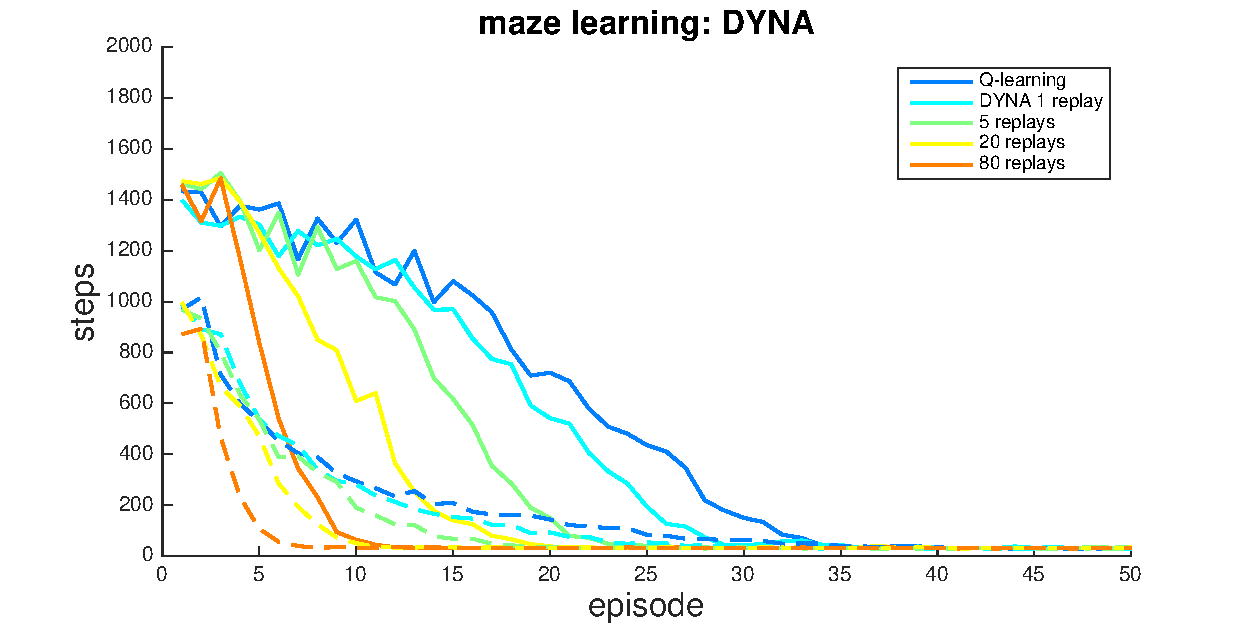
\includegraphics[width=\textwidth]{DYNAcompare}
\caption{The mean number of steps taken for 100 simulations of DYNA learning. The dense maze is shown in solid lines, while the sparse maze is shown in dashed lines. The convergence rate increases with the number of replays.}
\label{fig:dyna-compare}
\end{figure}

We next compare the performance of our two pseudoreward strategies in the presence of white noise (see Figure~\ref{fig:model-compare-noise}). For the dense maze (solid lines), we see that the Manhattan pseudoreward continues to fail to converge within 50 episodes in the presence of noise; because it had not converged without noise, this is unsurprising. The optimal policy reward plus noise also fails to converge to the optimal number of steps; however, it appears to reach a type of equilibrium (at least in this time frame) at around 1000 steps. Counterintuitively, adding DYNA replaying to this strategy actually \textit{worsens} performance; the mean number of steps stays at around 1900. We believe this is occurring because the DYNA planning stage after each step is reinforcing counterproductive behavior; DYNA adds more noise to an already noisy process.

For the sparse maze, adding white noise with $\sigma = 0.4$ to the pseudorewards prevents convergence to the true optimal value of 20 steps; both Manhattan and optimal policy pseudorewards seem to converge to about 200 steps. In this case, regular Q-learning and DYNA outperform noisy pseudorewards. Curiously, when DYNA replaying is combined with each of these noisy pseudorewards strategies, it drastically cuts performance--both pseudoreward strategies fail to converge and hover around 1500 steps. This is probably due to the fact that the DYNA replays are updating $Q(s,a)$ values for ``bad moves''; reinforcement learning is reinforcing the wrong thing.

\begin{figure}[ht]
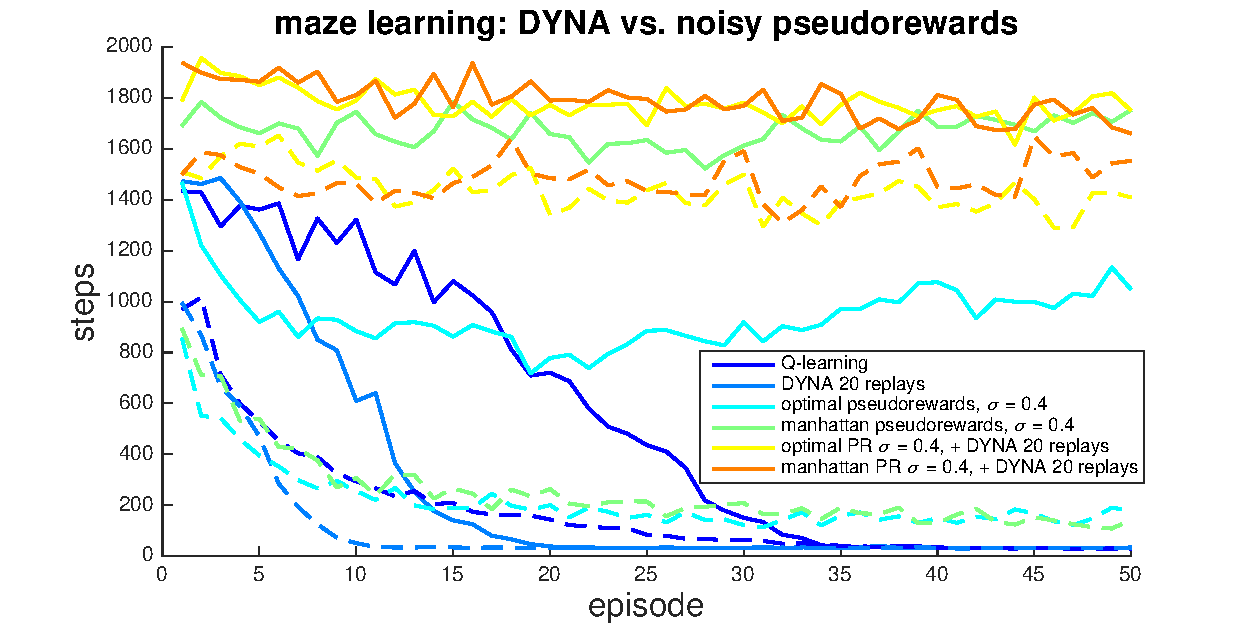
\includegraphics[width=\textwidth]{modelCompareHighNoise}
\caption{Pseudoreward learning under white noise with $\sigma = 0.4$ compared to Q-learning and DYNA learning. The mean number of steps taken for 100 simulations. The dense maze is shown in solid lines, while the sparse maze is shown in dashed lines.}
\label{fig:model-compare-noise}
\end{figure}

Finally, we explore how sensitive our pseudoreward methods are to various quantities of additive white noise, $\sigma$. For the dense maze, we see that the Manhattan pseudoreward does not converge for even $\sigma = 0$, while the optimal policy pseudoreward begins to not converge with noise level somewhere between $\sigma = 0.1$ and $\sigma = 0.4$. For the sparse maze, the pattern is clear: the more white noise is added, the the longer it takes for the pseudoreward learning method to converge.

\begin{figure}[ht]
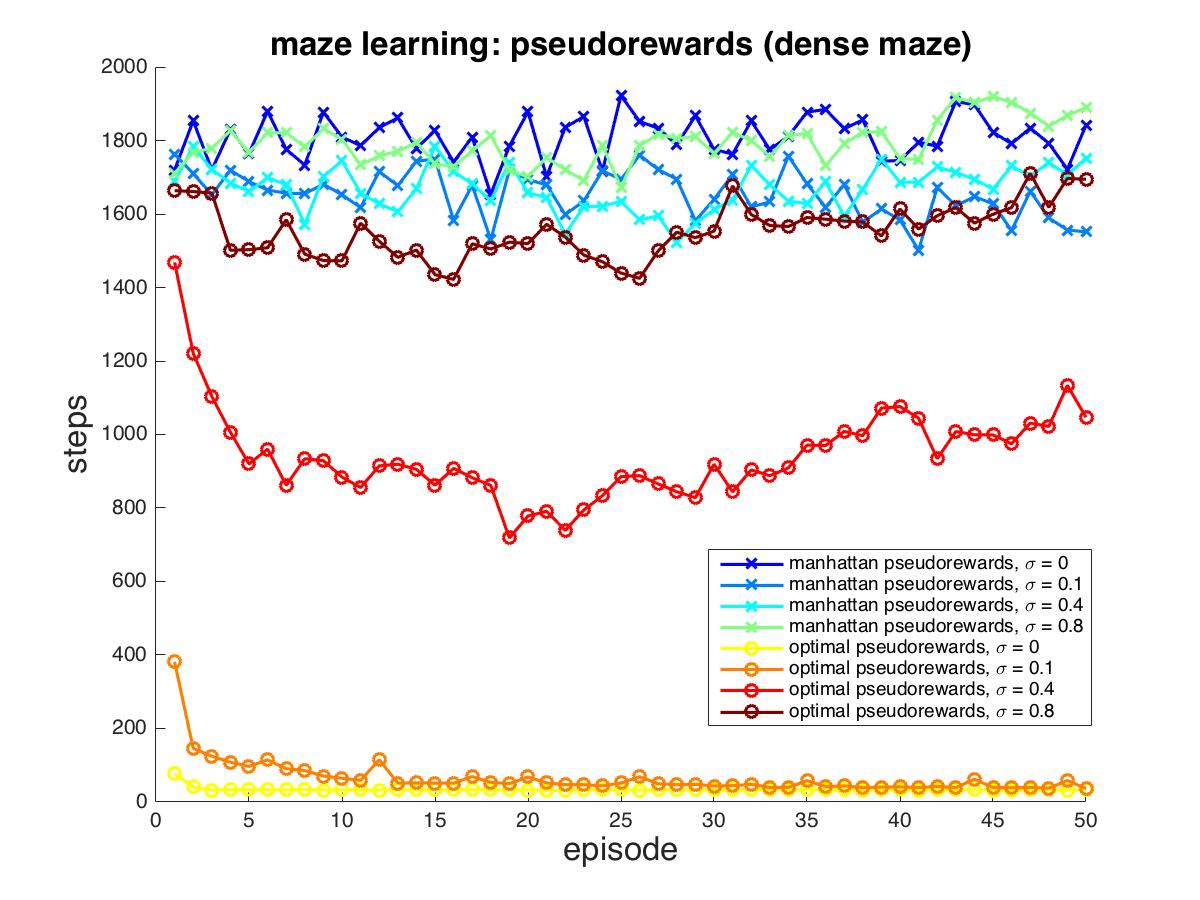
\includegraphics[width=0.9\textwidth]{PRdenseCompare}
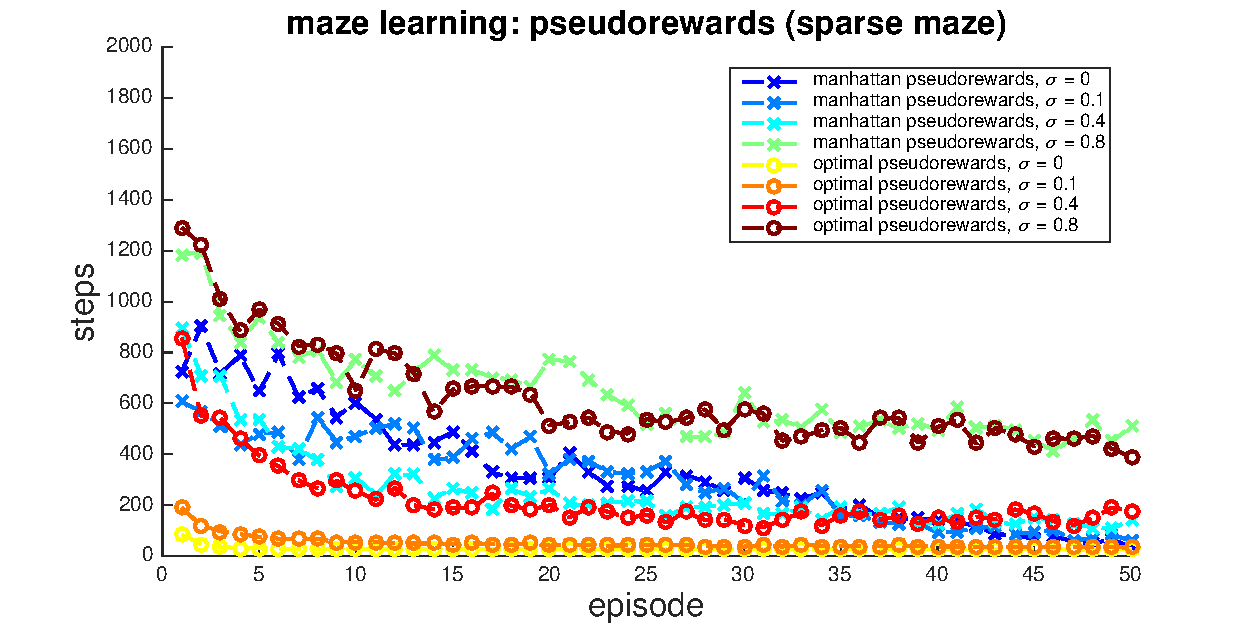
\includegraphics[width=0.9\textwidth]{PRsparseCompare}
\caption{Pseudoreward learning for each maze under various quantities of white noise, $\sigma = 0$ to $\sigma = 0.8$.}
\label{fig:sigma-compare}
\end{figure}

\section*{Discussion}

Our experiments compared three different types of RL algorithms: 1) simple Q-learning, 2) DYNA RL which combines Q-learning with model-based experience replay, 3) pseudorewards which modify model-free RL using a model-based system. We also tested a hybrid of DYNA and pseudoreward learning. Our results show that DYNA outperforms Q-learning in a maze-like environment, and optimal pseudorewards lead to the fastest convergence to optimal behavior. Furthermore, when optimal pseudorewards or manhattan heuristic pseudo rewards are combined with DYNA learning, the agent performs better than with either algorithm alone. However, when these pseudorewards become sufficiently noisey--which is more plausible in the real-world-- combining them with DYNA actually deteriorates performance, leading to less convergence or no convergence. The reason for this is that DYNA essentially magnifies the noise.

Researchers have for decades sought to understand how humans and even animals may construct a cognitive map versus using using simple model-free learning in maze environments~\cite{tolman1948cognitive,}. But there is little work studying how the two systems might cooperate. The algorithms we tested here could be used in a straightforward way to model the performance of humans or animals in a maze environment, in order to test which ones best match actual behavior. Furthermore, there is reason to believe that cognitive maps underlying spatial navigation, and the algorithms used to learn these maps, extent to other cognitive domains as well. Others have proposed that non-spatial maps are represented in a similar continuous space~\cite{buzsaki2013memory,tolman1948cognitive}, most famously in the case of episodic memory~\cite{o1978hippocampus}. Recent neural findings provide empirical support for this, and {behrens2015} found that cognitive maps of categories are represented in the brain using the same grid-based continuous spatial representations used for spatial navigation. This supports the fascinating hypothesis that humans may navigate through a virtual space of object representations when performing categorizations, akin to the way in which we find our way through physical space. It remains to be seen which other cognitive processes may be represented by similar space-like grids in the brain. While our maze environment ostensibly simulates spatial navigation, it's possible that it provides a strong analogy for other types of cognition as well.

Both DYNA learning and pseudorewards have recently been used as a framework for studying human learning and decision making. Evidence suggests that model-free and model-based RL systems interact in human learners~\cite{otto2013working,otto2013curse}, and that this interaction might be mediated by a DYNA architecture~\cite{gershman2014retrospective}. While the gamification framework has only recently been formalized as a framework for designing optimal incentive structures for human learners~\cite{lieder2016helping}, other findings could also be understood through the framework of pseudorewards, such as when human learners assign value to gaining information about their environment~\cite{wilson2014humans}. In none of these studies, however, has there been an explicit comparison between pseudorewards and DYNA, to test which one better models the data. Our experiments are the first data that we are aware of to explicitly compare the two.

Future work should investigate how humans implement pseudorewards, and how they learn such values. Affective responses are one plausible mechanism by which pseudorewards could be instantiated. Certain emotions could be used as a means of biasing an agent to make certain deicisions, and these emotions could be either built-in through evolution, learned from experience, or both. While many affective biases are known to sway humans away from optimal decision making~\cite{kahneman1979prospect}, more recent descriptions depict the rationality of these processes~\cite{griffiths2008bayesian}. One study has examined the interaction between emotional and rational/cognitive processing in the context of moral decision-making, linking these dual processes to model-free and model-based systems~\cite{cushman2013action}. While these authors suggest that emotions form the basis for the model-free component of these systems, within the context of pseudorewards is seems plausible that emotions could themselves be used to shape a model-free decision process. Within the context of moral decision making, for example, the emotion of remorse might function as a pseudoreward to retrain instinctive responses, making the agent more likely to behave within an ethical framework. The question of how pseudorewards are instantiated under different types of decision making, and how they interact with model-free RL, is a rich topic for future work.

More work should also be done to study how past experience and memories might be used to shape model-free RL, using the DYNA framework. Such work may elucidate how it is applied algorithmically or implemented biologically in humans or animals. One study provides indirect support for the implementation of DYNA in humans~\cite{gershman2014retrospective}, but this study did not compare DYNA with other potential mechanisms of cooperation between model-based and model-free RL, such as pseudorewards. While both forms of RL have proved valuable in modeling human and animal behavior, a systematic, model-comparison approach to studying alternative ways in which the systems may interact, remains under explored. Here we compared two such alternative models of this interaction. While our benchmarks use a maze setting, a next simple step would be to apply them to other decision making environments that are directly germane to particular questions of interest in cognition.

\section*{References}

\bibliography{final_report}{}
\bibliographystyle{apalike}

\end{document}